\section{Compression attacks}\label{sec:attack}

\subsection{A high-level overview}\label{subsec:example}
As explained above, compression side-channel attacks pose a serious threat
against real-world deployments of TLS and in general of any encryption system.
Although widely received and documented by the security community, there are
still not many existing mitigation strategies to thwart them, primarily due to
(i) the perceived high performance penalty associated with mitigating them, and
(ii) the perceived complexity and the lack of production code tools to allow for
the robust execution of such attacks. In this work we illustrate that these
perceptions are wrong and the continuous existence of such realistic threats
suggests a grave situation that needs to be addressed.

In order to appreciate the seriousness of these attacks we present a high-level
overview. Suppose that a user browses the Internet and accesses a website, like
a social network or a similar service that handles sensitive private data. When
the server receives a request for a page it collects all needed data, generates
the HTML code for the page and sends a network response containing this HTML.
All response data is encrypted under TLS, which ensures privacy and integrity
for the communication between the user and the server, and compressed for
efficiency.

Consider now an adversary that aims to break this communication's security.
This adversary tries to decrypt parts of the communication and reveal
information about the exchanged private data. However, in order to mount a
compression side-channel attack certain conditions need be met.

Firstly, we assume that the adversary is able to handle the user's network
traffic. That way he is able to collect and analyze the network packets of the
encrypted communication with the server.

Secondly, he is able to issue any number of malicious requests using the user's
cookies (which will be encrypted). This can be achieved by forcing the user's
browser to run a piece of code, such as a Javascript script. This script can be
either hosted on an adversary-controlled website or injected in plain HTTP
responses from third websites. This script is executed when loaded in the user's
browser and issues requests to any URL crafted by the adversary. Figure
\ref{fig:attack_model} elaborates further on this attack mode.

Thirdly, the web service under attack should allow data injection in the
encrypted response plaintext. This data takes the form of a specially crafted
``reflection'' string included in the malicious requests.

As the attack progresses the adversary collects network data containing multiple
reflections. Although this data is encrypted, analysis on the lengths of
different response packets in conjunction with the used reflection sequence will
reveal otherwise hidden properties of the private data. We will elaborate on the
analysis in section \ref{subsec:rupture}.

At this point the privacy of the communication between the user and the website
is compromised and the adversary has broken the confidentiality of the messages
by effectively circumventing TLS security.

    \begin{figure}[thpb]
        \centering
            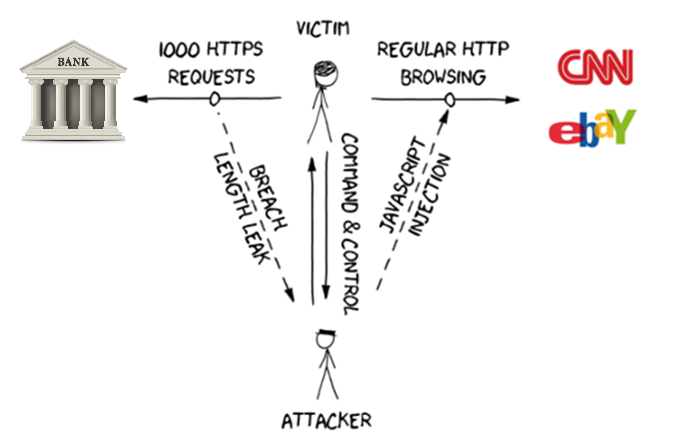
\includegraphics[width=0.48\textwidth]{figures/attack_model.png}
        \caption{The attack model}
        \label{fig:attack_model}
    \end{figure}

\subsection{A motivating example, concepts and notations}\label{subsec:terms}
We now describe a concrete example of the website in the previous section to
illustrate the various terms we use in the rest of this paper.

The target of the attack is the mail service found in the URL
\textit{mail.example.com}. The victim is the user that is logged in this service
and whose cookies are used in the malicious requests.

The web page that the adversary exploits is
\textit{mail.example.com/search?query=attack}. This website provides the HTTP
GET parameter \textit{query} and the adversary uses the reflection string
\textit{attack}. The HTML response is:

\begin{lstlisting}[basicstyle=\small\ttfamily]
<div>
    <p>You searched for: attack</p>
    <p>No results found.</p>
</div>
<div>
    Your inbox:
    <ul>
    <li>[Bank] Routing number: 123</li>
    </ul>
</div>
\end{lstlisting}

The server's HTML generator is an instance of the \textit{rendering function}
$f$. The output of $f$ is the \textit{rendered message} $m$, in our example the
HTML response.

The response contains multiple data elements. A data element can be a
\textit{secret}, \textit{static}, or a \textit{reflection}.

A \textit{secret} $s$ is any part of the response that the application wishes to
keep private. Examples of secrets include private messages, financial data, and
web security elements like CSRF tokens \cite{de2011automatic}. In our example,
the strings ``Bank", which is an email topic, and ``Routing number: 123", which
is the email body, are both secrets.

\textit{Static} is any content that remains unchanged across requests. Typical
examples of static data is HTML code, like ``div" or ``Your inbox:" in our
example. Static content is predictable and thus irrelevant to the attack.

A \textit{reflection} $r$ is a component crafted by the attacker that can be
adaptively transformed as the attack progresses. In this case, the HTTP GET
value ``attack" is a reflection. This string is included in the response in ``You
searched for: attack", an information message for the user reflected in every
search request.

Secrets are chosen from the distribution $\mathcal{M}$, which contains here all
routing numbers and 4-letter strings like ``Bank".

The compression function $\textrm{Com}$ is the compression algorithm used on the
HTML response plaintext. In our example, this algorithm is DEFLATE, the most
common compression algorithm on the web.

The encryption function $\textrm{Enc}$ is the encryption algorithm used by the
web server, the most common algorithm today being AES.  We use the function
$\mathcal{E}$ to describe the composition of $\textrm{Enc}$ and $\textrm{Com}$.

The input of $\mathcal{E}$ is the compression of $m$ and its output is the
ciphertext $c$ that is sent in the response packets and is sniffed by the
adversary over-the-wire.

The adversary issues the attack in stages. In each stage he creates a pool of
reflections and makes malicious requests for each reflection in the pool. An
attack stage ends when the adversary has successfully decrypted a single
character in the secret.
